\chapter{Curva caracteristica de los diodos}

\section{Activida de simulacion}

\subsection{Polarizacion en directa}

\subsection{Polarizacion en inversa}

\section{Actividad de laboratorio}

\begin{figure}[H]
  \centering
  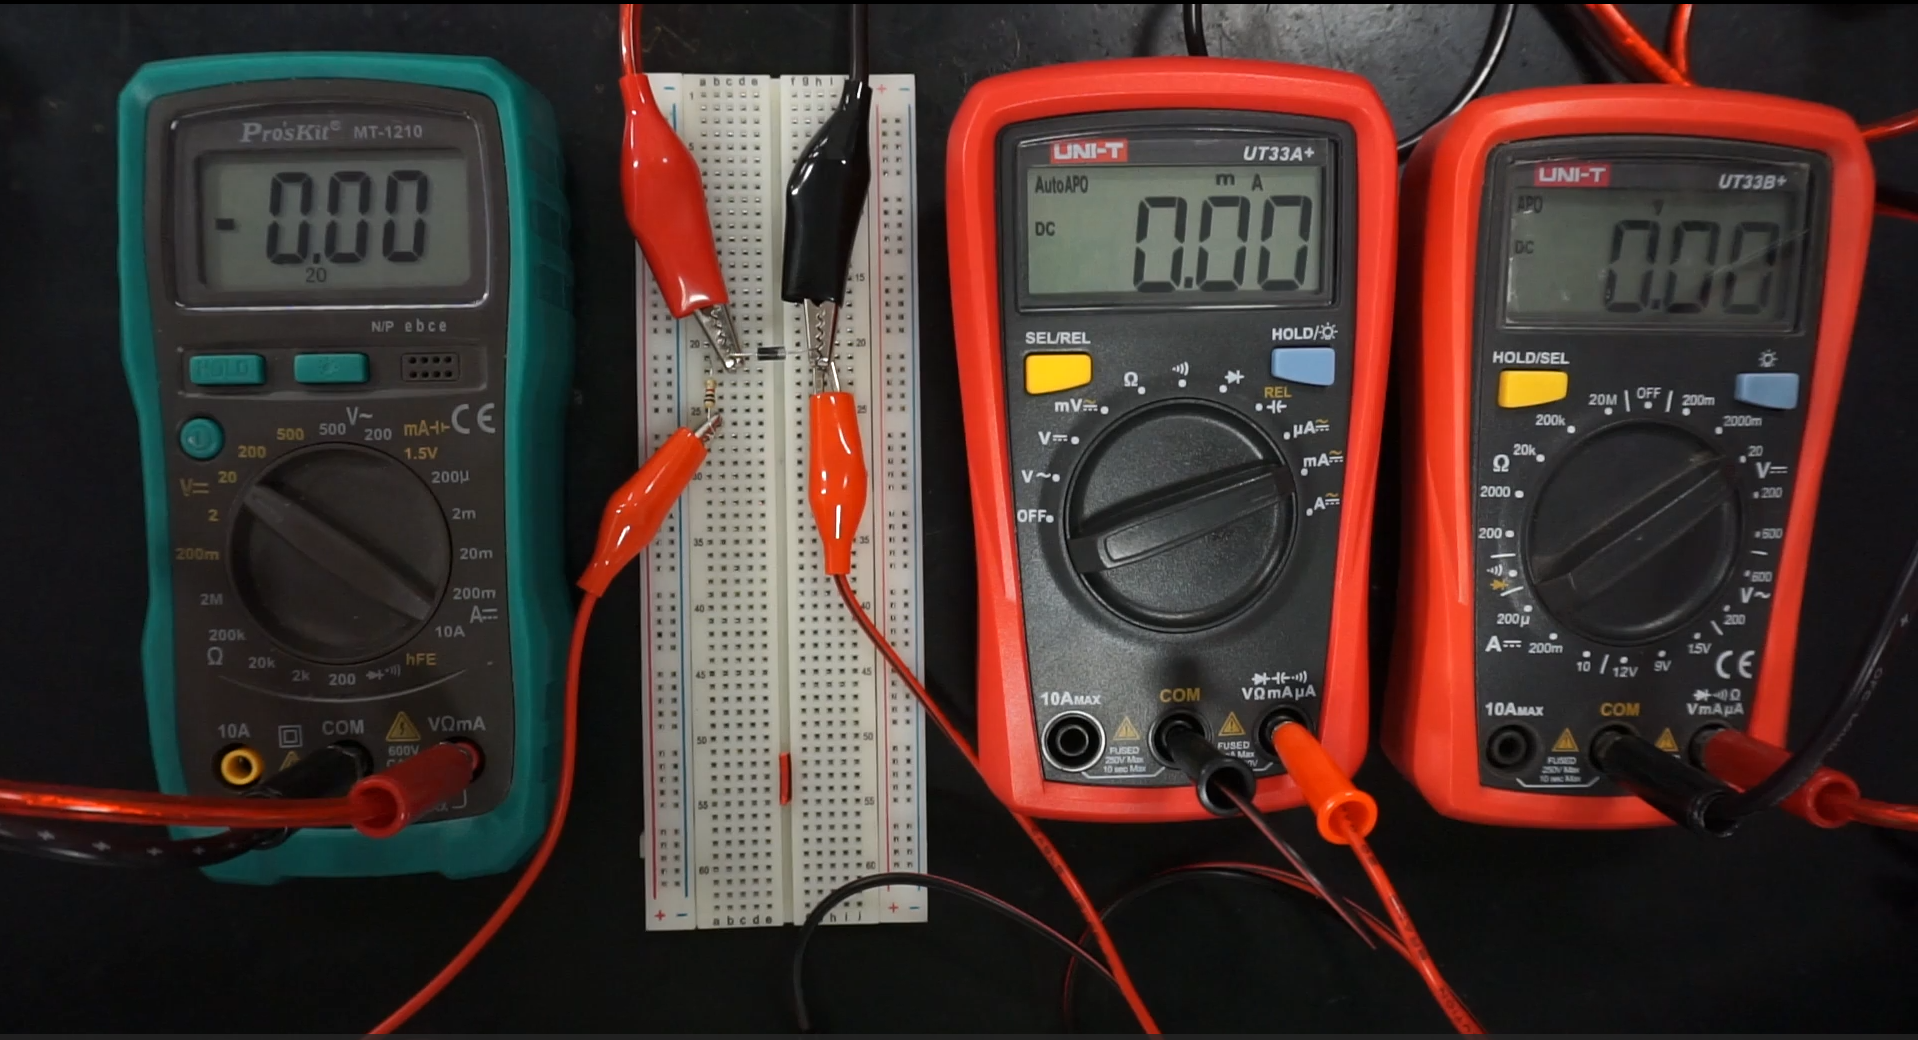
\includegraphics[width=0.7\textwidth]{images/circuitoN4007.png}
  \caption{Circuito del diodo 1N4007 en polarizacion directa}
\end{figure}

\begin{figure}[H]
  \centering
  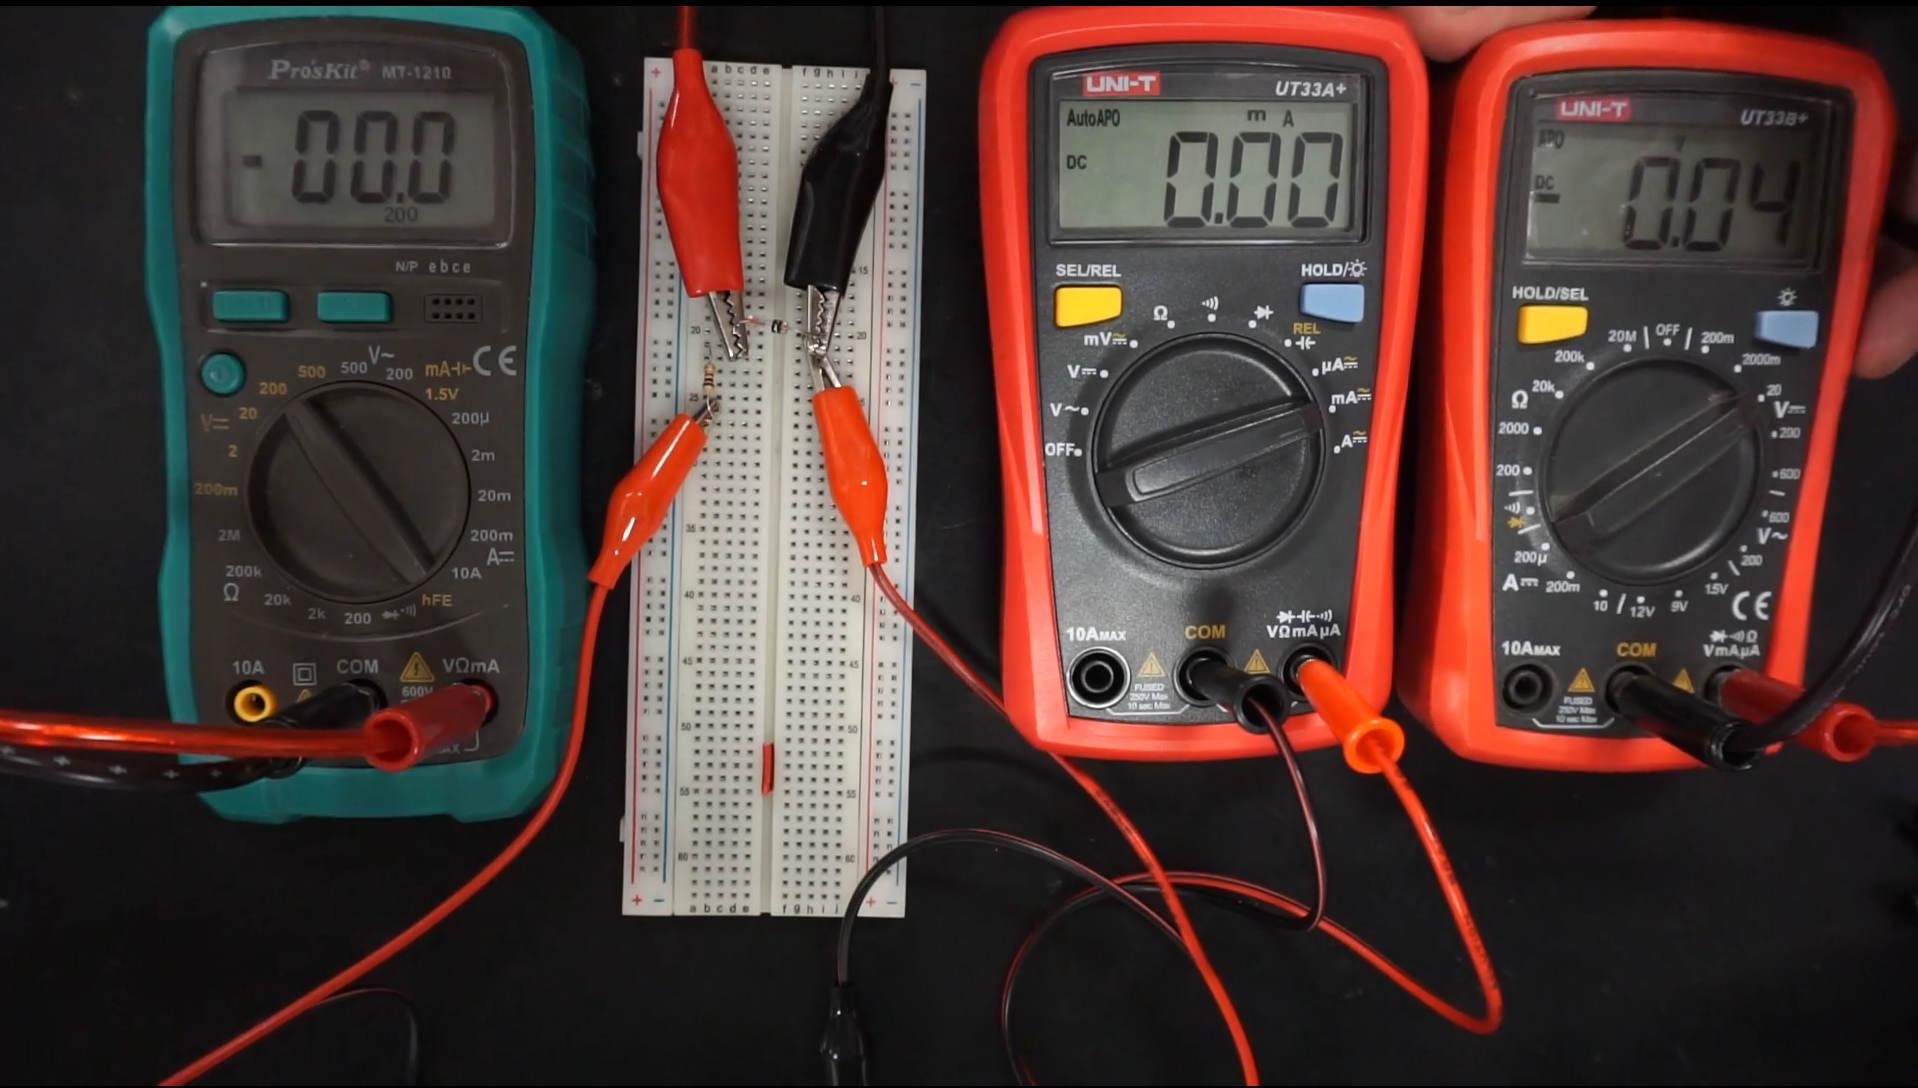
\includegraphics[width=0.7\textwidth]{images/circuitoN60.png}
  \caption{Circuito del diodo 1N60 en polarizacion directa}
\end{figure}

\begin{table}[H]
  \begin{tabular}{|c|c|c|c|c|c|c|c|c|c|c|c|c|c|}
    \hline
    $V_1$[V] & 0 & 0,1 & 0,3 & 0,4 & 0,45 & 0,5 & 0,55 & 0,6 & 0,65 & 0,7 & 1 & 3 & 5
    \hline
    $V_D$[V] & 0 & 0,19 & 0,24 & 0,31 & & & & & & & & & &
    \hline
    $I_D$[\mA] & 0 & 0 & 0 & & 0 &  & & & & & & & &
    \hline
  \end{tabular}
  \caption{Tabla datos obtenidos en el diodo 1N4007}
\end{table}

